\chapter{Parameter estimation and Galactic bursts\label{ch:param}}

Extreme-mass-ratio bursts could provide a means of investigating the properties of MBHs with a space-borne detector. In the previous chapter we constructed approximate burst waveforms. We now begin to investigate their properties. To be useful for astronomy EMRBs must be: (i) detectable, (ii) informative and (iii) likely to happen. If bursts are not detectable, they can be of no use. If they are detectable but not informative, then at best they could only tell us that there are objects on highly eccentric orbits. This could be interesting if we observe enough to do statistics, but this depends upon the event rate. If the event rate is too low, then even if EMRBs are wonderfully informative they are unlikely to be of practical use. EMRBs must fulfill all three criteria to be a viable tool for learning about MBHs.

In this chapter we start to address the first two criteria. We begin by concentrating on the Galaxy's MBH; as it is our local MBH, it is the most promising candidate. In \secref{Waveforms} we look at our NK waveforms and determine that they could be detectable. We give fiducial power-law fits for SNR as a function of periapse radius, which are useful for back-of-the-envelope estimates. We explain how to extract the information from the bursts in \secref{Estimation}. Results estimating the measurement precision are then presented in \secref{Gal-Results}.

%In the following chapter we go on to consider extragalactic sources. These are not as promising as the GC, but could still contribute to the total burst event rate. We address the question of event rates in ... where we construct a model for our Galaxy.

\section{Waveforms and detectability}\label{sec:Waveforms}

\subsection{Model parameters}\label{sec:Mod-param}

The waveform depends on the properties of the MBH; the CO and its orbit, and the detector. We assume the position of the detector is known. This is specified by $\overline{\phi}$ and $\varphi$. We chose the initial position so $\overline{\phi} = 0$ when $\varphi = 0$ \citep{Cutler1998}; this does not qualitatively influence our results.\footnote{See \citet{Jani2013} for a discussion of the possibilities for optimising the choice of the initial phase.}

We also treat the sky position of the MBH, given by $\overline{\Theta}$ and $\overline{\Phi}$, as known. These are taken as the coordinates of Sgr A*, as the radio source is expected to be within $20 r\sub{g}$ of the MBH \citep{Reid2003,Doeleman2008}. We use the J2000.0 coordinates \citep{Reid1999, Yusef-Zadeh1999}. These change with time due to the rotation of the SS about the GC; the proper motion is about $6\units{mas\,yr^{-1}}$, mostly in the plane of the galaxy \citep{Reid1999, Backer1999, Reid2003}. The position is already determined to high accuracy and an EMRB can only give weak constraints on source position, hence we shall not try to infer it.\footnote{For comparison, an EMRI, which should be more informative, can only give sky localisation to $\sim 10^{-3}~\mathrm{steradians}$ \citep{Barack2004, Huerta2009}.}

For our model, the input parameters left to infer are:
\begin{enumerate}[leftmargin=*, widest=\:88--88.]
\item[1.] The MBH's mass $M_\bullet$. This is currently well constrained by the observation of stellar orbits about Sgr A* \citep{Ghez2008, Gillessen2009}, with the best estimate being $M_\bullet = (4.31 \pm 0.36) \times 10^6 M_\odot$. This depends upon the galactic centre distance $R_0$ as $M_\bullet = (3.95 \pm 0.06|\sub{stat} \pm 0.18|_{R_0, \, \mathrm{stat}} \pm  0.31|_{R_0, \, \mathrm{sys}}) \times 10^6 M_\odot (R_0 / 8\units{kpc})^{2.19}$, where the errors are statistical, independent of $R_0$; statistical from the determination of $R_0$, and systematic from $R_0$ respectively.
\item[2.] The spin parameter $a_\ast$. Naively this could be anywhere in the range $|a_\ast| < 1$; however it is possible to place an upper bound by contemplating spin-up mechanisms. Considering the torque from radiation emitted by an accretion disc, and swallowed by a BH, it can be shown that $|a_\ast| \lesssim 0.998$ \citep{Thorne1974}. Magnetohydrodynamical simulations of accretion discs produce a smaller maximum value of $|a_\ast| \sim 0.95$ \citep{Gammie2004}. The actual spin value could be much lower than this upper bound depending upon the MBH's evolution.
\item[3, 4.] The orientation angles for the MBH spin $\Theta\sub{K}$ and $\Phi\sub{K}$. These are defined in the ecliptic coordinate system from \figref{SS_LISA}.
\item[5.] The ratio of the SS-GC distance $R_0$ and the CO mass $\mu$, which we denote as $\zeta = R_0/\mu$. This scales the amplitude of the waveform. Bursts, unlike inspirals, do not undergo orbital evolution, hence we cannot break the degeneracy in $R_0$ and $\mu$, and they cannot be inferred separately. The distance, like $M_\bullet$, is constrained by stellar orbits, the best estimate being $R_0 = 8.33 \pm 0.35\units{kpc}$ \citep{Gillessen2009}. The mass of the orbiting particle depends upon the type of object: whether it is an MS star, WD, NS or BH. Since we shall not know the $\mu$ precisely, we shall not be able to infer anything more about the distance to the GC.
\item[6, 7.] The angular momentum of the CO. This can be described using either $\{L_z, Q\}$ or $\{L_\infty, \iota\}$. We employ the latter, as the total angular momentum and inclination are less tightly correlated. Assuming spherical symmetry, we expect $\cos \iota$ to be uniformly distributed.
\item[8--10.] A set of coordinates to specify the trajectory. These could be positions at an arbitrary time. We use the angular phases at periapse, $\phi\sub{p}$ and $\chi\sub{p}$ (which determines $\theta\sub{p}$), as well as the time of periapse $t\sub{p}$.
\end{enumerate}
We are therefore interested in constraining $d = 10$ parameters. We shall use $\boldsymbol{\lambda}$ to represent the set of these $d$ parameters.

Of paramount importance are the mass and spin. Together, these fully describe the MBH, all the information regarding its formation and growth must be inferred from these parameters. As we have a good estimate of the mass, to gain a complete description of the MBH we have only to measure its spin; this shall give us insight into its history and role in the evolution of the Galaxy.

\subsection{Waveforms and kludge coordinates}\label{sec:wave-ex}

\Figref{Examples} shows example waveforms to demonstrate some of the possible variations in the signal. All these assume the standard mass and position for the MBH as well as a $\mu = 10 M_\odot$ orbiting CO; other (randomly chosen) orbital parameters are specified in the captions. Radii are given in terms of the gravitational radius $r\sub{g} = GM_\bullet / c^2$.
\begin{figure}%[!htp]
  \begin{center}
   \subfigure[{Waveform for $a_\ast \simeq 0.12$, $r\sub{p} \simeq 15.6 r\sub{g}$ and $\iota \simeq 2.1$. The SNR for the spherical polar kludge waveform (plotted) is $\rho[\boldsymbol{h}\sub{sph}] \simeq 451$, for the oblate-spheroidal kludge it is $\rho[\boldsymbol{h}\sub{ob}] \simeq 451$ (agreement to $0.01\%$).}]{\label{fig:Orbit_233} 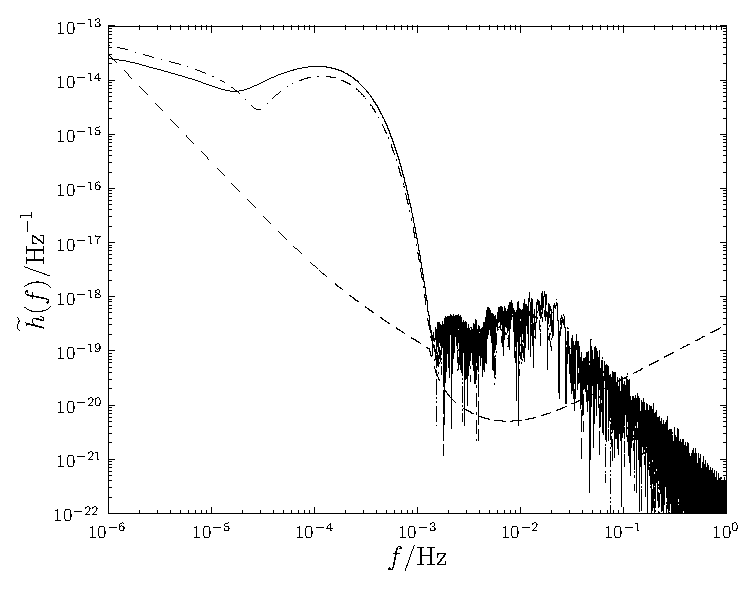
\includegraphics[width=0.47\textwidth]{./images/Fig_new_sph_h_233}} \quad
   \subfigure[{Waveform for $a_\ast \simeq 0.74$, $r\sub{p} \simeq 3.2 r\sub{g}$ and $\iota \simeq 1.2$. The SNR for the spherical polar kludge waveform (plotted) is $\rho[\boldsymbol{h}\sub{sph}] \simeq 70600$, for the oblate-spheroidal kludge it is $\rho[\boldsymbol{h}\sub{ob}] \simeq 74900$.}]{\label{fig:Orbit_135} 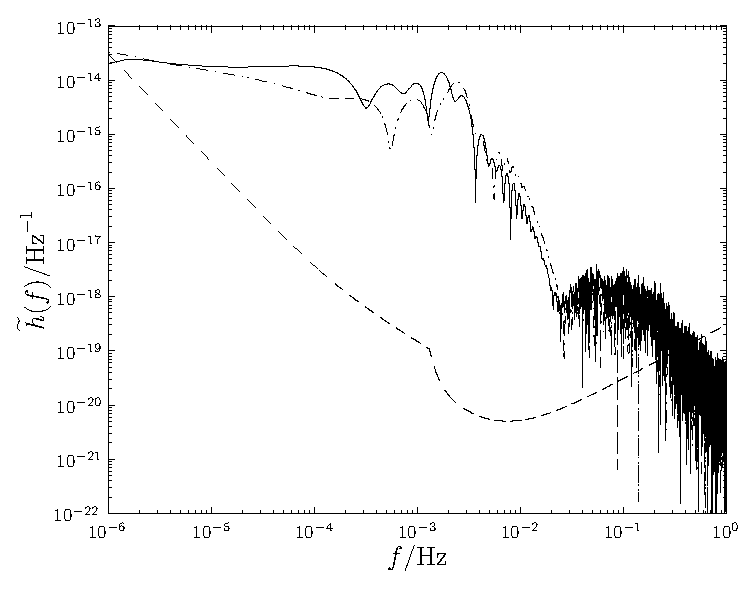
\includegraphics[width=0.47\textwidth]{./images/Fig_new_sph_h_135}}  
\caption{Example burst waveforms from the galactic centre. The strain $\widetilde{h}\sub{I}(f)$ is indicated by the solid line, $\widetilde{h}\sub{II}(f)$ by the dot--dashed line, and the noise curve by the dashed line. The kludge has been formulated using spherical polar coordinates.\label{fig:Examples}}
  \end{center}
\end{figure}

The plotted waveforms use the spherical polar coordinate system for the NK. Using oblate-spheroidal coordinates makes a small difference. On the scale shown here the only discernible difference would be in \figref{Orbit_135}; the maximum difference in that waveform (outside the high-frequency tail) is $\sim 10\%$. In the other cases the difference is entirely negligible (except in the high-frequency tail, which is not of physical significance). This behaviour is typical; for the closest orbits, with the most extreme spin parameters, the maximum difference in the waveforms may be $\sim 30\%$. The difference is largely confined to the higher frequency components, which are most sensitive to the parts of the trajectory closer to the MBH: the change in flat-space radius for the same Boyer--Lindquist radial coordinate causes a slight shift in the shape of the spectrum. Enforcing the same flat-space periapsis gives worse agreement across the spectrum.

To examine the effect of the coordinate choice, we compare SNRs calculated using the alternative schemes for a selection of orbits. The orbits have periapse distances uniformly distributed in log-space between the innermost orbit and $100 r\sub{g}$. Each had a spin and orbital inclination randomly chosen from distributions uniform in $a_\ast$ and $\cos \iota$.\footnote{The innermost orbit depends upon $a_\ast$ and $\iota$, hence these are drawn first.} For every periapse, five SNRs were calculated, each having a different set of ancillary parameters specifying the relative orientation of the MBH, the orbital phase and the position of the detector, drawn from appropriate uniform distributions. We take the mean of $\ln \rho$ for each set of ancillary parameters.\footnote{The logarithm is a better quantity to work with since the SNR is a positive-definite quantity that may be distributed over a range of magnitudes \citep[sections 22.1, 23.3]{MacKay2003}. Using median values yields results that are quantitatively similar.} The MBH parameters were fixed as for the GC.

The ratio of the two SNRs is shown in \figref{Oblate_sphere}.
\begin{figure}%[!htp]
\begin{center}
 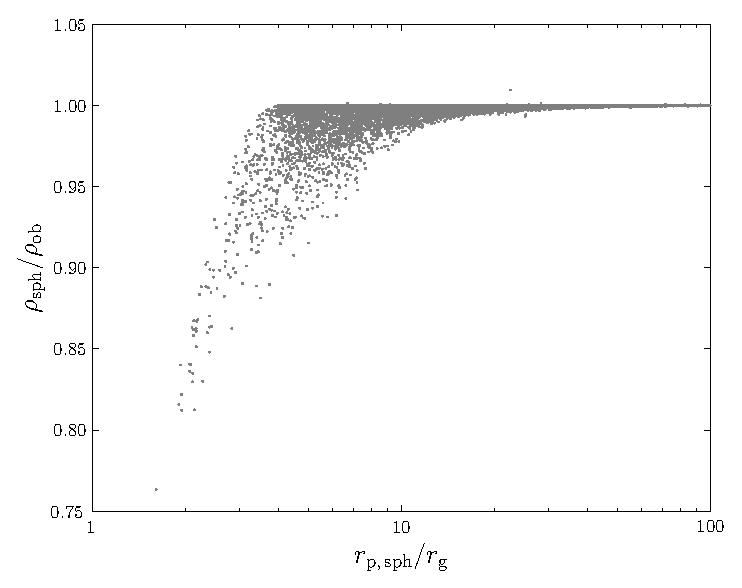
\includegraphics[width=0.6\textwidth]{./images/Fig_SNR_ratio}
 \caption{Ratio of SNR for a waveform calculated using spherical polar coordinates to that for a waveform using oblate-spheroidal coordinates.\label{fig:Oblate_sphere}}
   \end{center}
\end{figure}
The difference from the coordinate systems is only apparent for orbits with very small periapses. There is agreement to $10\%$ down to $r\sub{p} \simeq 4 r\sub{g}$; the maximal difference may be expected to be $\sim 20\%$, this is for periapses that are only obtainable for high spin values.

Since the deviation in the two waveforms is only apparent for small periapses, when the kludge approximation is least applicable, we conclude that the choice of coordinates is unimportant. The potential error of order $10\%$ is no greater than that inherent in the NK approximation (see \secref{Energy}). Without an accurate waveform template to compare against, we do not know if there is a preferable choice of coordinates. We adopt spherical coordinates for easier comparison with existing work.

\subsection{Signal-to-noise ratios}\label{sec:Gal-SNR}

The detectability of a burst depends upon its SNR. To characterise the variation of $\rho$ we calculated SNRs for a range of orbits. These were generated as in \secref{wave-ex}, we used $\sim 10^4$ different periapse distances.

The bursts were calculated for a $1 M_\odot$ CO. From \eqnref{octupole}, the amplitude of the waveform is proportional to the CO mass $\mu$, and so $\rho$ is also proportional to $\mu$; a $10 M_\odot$ object would be ten times louder on the same orbit. To make results mass independent, we work in terms of a mass-normalised SNR
\begin{equation}
\hat{\rho}[\boldsymbol{h}] = \left(\frac{\mu}{M_\odot}\right)^{-1}\rho[\boldsymbol{h}].
\end{equation}

There exists a correlation between the periapse radius and SNR, as shown in \figref{SNR}.
\begin{figure}%[!htp]
  \begin{center}
  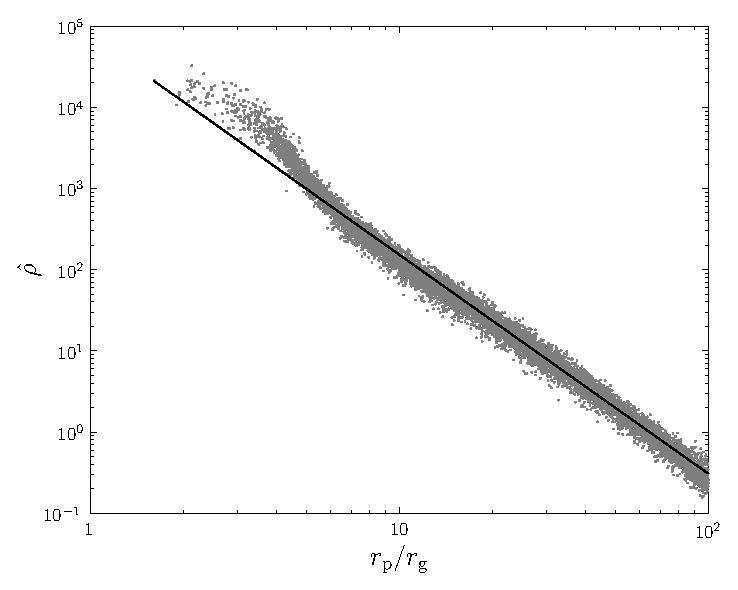
\includegraphics[width=0.6\textwidth]{./images/Fig_SNR}
    \caption{Mass-normalised SNR as a function of periapse radius for LISA. The plotted points are the values obtained by averaging over each set of ancillary parameters. The best fit line is $\log(\hat{\rho}) = -2.69\log(r\sub{p}/r\sub{g}) + 4.88$. This is fitted to orbits with $r\sub{p} >  13.0 r\sub{g}$.\label{fig:SNR}} % and has a reduced chi-squared value of $\chi^2/\nu = 1.73$
  \end{center}
\end{figure}
Closer orbits produce louder bursts. To reflect this trend, we have fitted a simple fiducial power law,
\begin{equation}
\log\rho \simeq -2.7\log\left(\frac{r\sub{p}}{r\sub{g}}\right) + \log\left(\frac{\mu}{M_\odot}\right) + 4.9,
\label{eq:SNR-power-law}
\end{equation}
which is indicated by the straight line.\footnote{Using oblate-spheroidal coordinates instead of spherical polars gives a fit consistent to within $0.1\%$ as we have excluded the closest orbits.} This was done by maximising the likelihood, assuming $\ln \rho$ has a Gaussian distribution with standard deviation derived from the scatter because of variation in the ancillary parameters. The power law is a good fit only for larger periapses. The shape is predominately determined by the noise curve. The change in the trend reflects the transition from approximately power law behaviour to the bucket of the noise curve. Hence, we fit a power law to orbits with a characteristic frequency of $f_\ast = \sqrt{GM_\bullet/r\sub{p}} < 1 \times 10^{-3}\units{Hz}$, to avoid spilling into the bucket.\footnote{The form of $f_\ast$ can be derived on dimensional grounds, but it is explained in more detail in \secref{extragal-SNR}.} Changing the cut-off within a plausible region alters the fit coefficients by around $0.1$.\footnote{The power law exponent $-2.7$ is inconsistent with $-13/4$ as predicted by the approximate model of \citet{Hopman2007}. This is the result of their approximate waveform model.}

The SNR shows no clear correlation with the other parameters (excluding $\mu$). However, the SNR is sensitive to the orbital parameters, in particular the initial position, and may vary by an order of magnitude.

Setting a threshold of $\rho = 10$, a $1 M_\odot$ ($10 M_\odot$) object would be expected to be detectable if the periapse distance is less than $27 r\sub{g}$ ($65 r\sub{g}$). \citet{Hopman2007}, assuming a threshold of $\rho = 5$, used an approximate form for the SNR based upon the quadrupole component of a circular orbit; their model, with updated parameters for the MBH, predicts bursts would be detectable out to $66 r\sub{g}$ ($135 r\sub{g}$). This is overly optimistic.

Following a similar approach, we may repeat this analysis for eLISA. The SNR as a function of periapse is shown in \figref{SNR-eLISA}.
\begin{figure}%[!htp]
  \begin{center}
  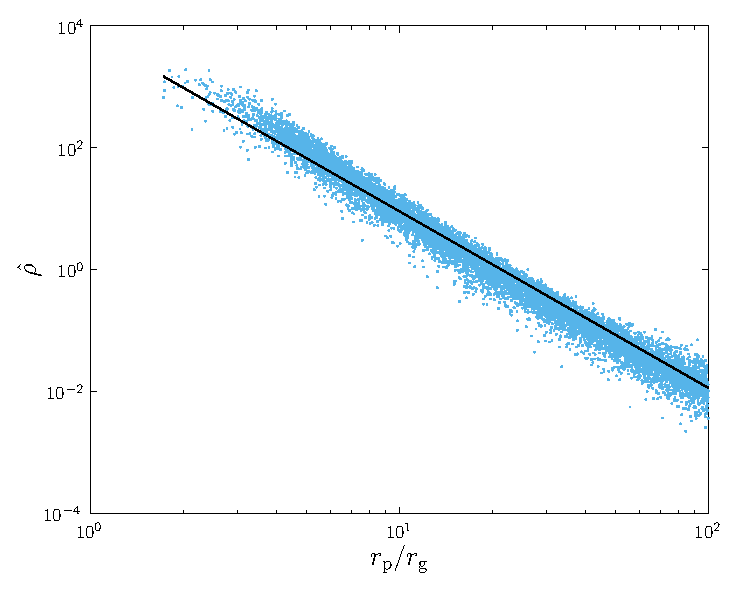
\includegraphics[width=0.6\textwidth]{./images/Fig_SNR_eLISA_NGO}
    \caption{Mass-normalised SNR as a function of periapse radius for eLISA. The plotted points are the values obtained by averaging over each set of ancillary parameters. The best fit line is $\log(\hat{\rho}) = -2.90\log(r\sub{p}/r\sub{g}) + 3.85$. This is fitted to orbits with $r\sub{p} >  13.0 r\sub{g}$.\label{fig:SNR-eLISA}}
    \end{center}
\end{figure}
There is again a strong correlation that may be approximated as a power law. The bucket of the noise curve is less apparent as it is shifted to slightly higher frequencies. We have fitted
\begin{equation}
\log\rho \simeq -2.9\log\left(\frac{r\sub{p}}{r\sub{g}}\right) + \log\left(\frac{\mu}{M_\odot}\right) + 3.9,
\label{eq:SNR-power-law-eLISA}
\end{equation}
which is indicated by the straight line. This was done in exactly the same as for LISA. Again, there is no clear correlation with any other orbital parameters.

The SNR is lower for eLISA. As a consequence, bursts are detectable across a smaller range of periapses. Using the threshold $\rho = 10$, a $1 M_\odot$ ($10 M_\odot$) object would be expected to be detectable if the periapse distance is less than $10 r\sub{g}$ ($21 r\sub{g}$). This is a reduction of about a factor of three compared to LISA.

\section{Parameter estimation}\label{sec:Estimation}

Having detected a signal, we are interested in what we can learn about the source. We have an inference problem that can be solved by an application of Bayes' Theorem \citep[chapter 4]{Jaynes2003}: the probability distribution for our parameters given that we have detected the signal $\boldsymbol{s}(t)$ is given by the posterior
\begin{equation}
p(\boldsymbol{\lambda}|\boldsymbol{s}(t)) = \frac{p(\boldsymbol{s}(t)|\boldsymbol{\lambda})p(\boldsymbol{\lambda})}{p(\boldsymbol{s}(t))}.
\end{equation}
Here $p(\boldsymbol{s}(t)|\boldsymbol{\lambda})$ is the likelihood of the parameters, $p(\boldsymbol{\lambda})$ is the prior probability distribution for the parameters, and the evidence $p(\boldsymbol{s}(t)) = \intd{}{}{p(\boldsymbol{s}(t)|\boldsymbol{\lambda})}{^d \lambda}$ is, for our purposes, a normalising constant. The likelihood depends upon the realization of noise. If parameters $\boldsymbol{\lambda}_0$ define a waveform $\boldsymbol{h}_0(t) = \boldsymbol{h}(t; \boldsymbol{\lambda}_0)$, the probability that we observe signal $\boldsymbol{s}(t)$ GW is given by \eqnref{sig_prob}, so the likelihood is
\begin{equation}
p(\boldsymbol{s}(t)|\boldsymbol{\lambda}_0) \propto \exp\left[-\recip{2}\innerprod{\boldsymbol{s}-\boldsymbol{h}_0}{\boldsymbol{s}-\boldsymbol{h}_0}\right].
\label{eq:likelihood}
\end{equation}
If we were to define this as a probability distribution for the parameters $\boldsymbol{\lambda}$, the modal values are the maximum-likelihood (ML) parameters $\boldsymbol{\lambda}\sub{ML}$. The waveform $\boldsymbol{h}(t; \boldsymbol{\lambda}\sub{ML})$ is the signal closest to $\boldsymbol{s}(t)$, where distance is defined using the inner product (\ref{eq:inner}) \citep{Cutler1994}.

To discover if any parameters can be accurately inferred, we must characterise the form of the posterior. We discuss two approaches for mapping the shape of the posterior: Fisher matrices and Markov chain Monte Carlo (MCMC) sampling.

\subsection{Fisher matrices}\label{sec:Fisher}

In the limit of a high SNR, we may approximate \citep{Vallisneri2008}
\begin{equation}
p(\boldsymbol{s}(t)|\boldsymbol{\lambda}_0) \propto \exp\left[-\recip{2}\innerprod{\partial_a\boldsymbol{h}}{\partial_b\boldsymbol{h}}\left(\lambda^a - \langle\lambda^a\rangle_\ell\right)\left(\lambda^b - \left\langle\lambda^b\right\rangle_\ell\right)\right],
\label{eq:LSA}
\end{equation}
where the mean is defined as
\begin{equation}
\langle\lambda^a\rangle_\ell = \frac{\intd{}{}{\lambda^a p(\boldsymbol{s}(t)|\boldsymbol{\lambda})}{^d \lambda}}{\intd{}{}{p(\boldsymbol{s}(t)|\boldsymbol{\lambda})}{^d \lambda}}.
\end{equation}
In the high SNR limit, this is the ML value $\langle\lambda^a\rangle_\ell = \lambda^a\sub{ML}$. The quantity
\begin{equation}
\Gamma_{ab} = \innerprod{\partial_a\boldsymbol{h}}{\partial_b\boldsymbol{h}}
\label{eq:Fisher}
\end{equation}
is the Fisher information matrix (FIM). It controls the variance of the likelihood distribution.

The form of the posterior distribution depends upon the nature of the prior information. If we have an uninformative prior, such that $p(\boldsymbol{\lambda})$ is a constant, the posterior distribution is determined by the likelihood. In the high SNR limit, we obtain a Gaussian with variance-covariance matrix
\begin{equation}
\boldsymbol{\Sigma} = \boldsymbol{\Gamma}^{-1}.
\label{eq:InvFisher}
\end{equation}
The FIM therefore gives the uncertainty associated with the inferred parameters, in this case the ML values.

If the prior restricts the allowed range for a parameter, as is the case for the spin $a_\ast$, then the posterior is a truncated Gaussian, and $\boldsymbol{\Gamma}^{-1}$ may no longer represent the variance-covariance.

If the prior is approximately Gaussian with variance-covariance matrix $\boldsymbol{\Sigma}_0$, the posterior is also Gaussian.\footnote{If we only know the typical value and spread of a parameter, a Gaussian is the maximum entropy prior (\citealt{Jaynes2003}, section 7.11): the prior that is least informative given what we know.} The posterior variance-covariance is \citep{Cutler1994, Vallisneri2008}
\begin{equation}
\boldsymbol{\Sigma} = \left(\boldsymbol{\Gamma} + \boldsymbol{\Sigma}_0^{-1}\right)^{-1}.
\label{eq:Posterior_variance}
\end{equation}
From this the inverse FIM $\boldsymbol{\Gamma}^{-1}$ is an upper bound on the size of the posterior covariance matrix.\footnote{It is also the Cram\'{e}r-Rao bound on the error covariance of an unbiased estimator \citep{Cutler1994, Vallisneri2008}. Thus it represents the frequentist error: the lower bound on the covariance for an unbiased parameter estimator $\boldsymbol{\lambda}\sub{est}$ calculated from an infinite set of experiments with the same signal $\boldsymbol{h}(t)$ but different realisations of the noise $\boldsymbol{n}(t)$.}

The FIM gives a quick way of estimating the range of the posterior. It is widely used because of this. However, it is only appropriate when the approximation of \eqnref{LSA} holds. This is known as the linearised-signal approximation (LSA), where higher order derivatives are neglected. To assess the validity of this, \citet{Vallisneri2008} recommends use of the maximum-mismatch (MM) criterion
\begin{equation}
\ln r = -\recip{2}\innerprod{\Delta\lambda^a\partial_a\boldsymbol{h}\sub{ML} - \Delta\boldsymbol{h}}{\Delta\lambda^b\partial_b\boldsymbol{h}\sub{ML} - \Delta\boldsymbol{h}}.
\end{equation}
Here $\Delta \boldsymbol{\lambda}$ is the displacement to some point on the $1\sigma$ surface
\begin{equation}
\Delta \boldsymbol{\lambda} = \boldsymbol{\lambda}\sub{1\sigma} - \boldsymbol{\lambda}\sub{ML},
\end{equation}
and $\Delta \boldsymbol{h}$ is the corresponding change in the waveform
\begin{equation}
\Delta \boldsymbol{h} = \boldsymbol{h}(\boldsymbol{\lambda}\sub{1\sigma}) - \boldsymbol{h}(\boldsymbol{\lambda}\sub{ML}).
\end{equation}
The $1\sigma$ surface is defined from the inverse of the FIM. If higher order terms are indeed negligible, the MM criterion is small. We check this by picking a random selection of points on the $1\sigma$ surface and evaluating $|\ln r|$. If this is smaller than a fiducial value ($|\ln r| = 0.1$) over the majority ($90\%$) of the surface we consider the LSA sufficiently justified.

We calculated FIMs for a wide range of orbits and checked the MM criterion. We found that for the overwhelming majority the test failed: the LSA is not appropriate. This behaviour was seen even for orbits with $\rho \sim 10^3$--$10^4$.\footnote{In this study, to increase $\rho$ we must reduce the periapse distance; this also reduces the region where the LSA is valid as parameter dependencies become more non-linear. If we had the luxury of increasing $\rho$ by moving the GC closer, things could be different.} Higher order terms are important, and cannot be neglected.

EMRBs have a short duration and accordingly are not the most informative of signals. Therefore, the $1\sigma$ surface as defined by considering only the LSA terms is large. Taking such a step in parameter space moves the signal beyond the region of linear changes.

What constitutes high SNR depends upon the signal; it is not enough for $\rho > 1$. As stressed by \citet{Vallisneri2008}, it is essential to check the MM criterion for individual waveforms: the threshold for the LSA to become applicable could be much greater than naively thought.

As we cannot be confident in FIM results, we abandon this approach in favour of using Markov chain Monte Carlo simulations to explore constraints from different regions of parameter space. These are computationally more expensive, but do not rely on any approximations.

\subsection{Markov chain Monte Carlo methods}\label{sec:MCMC}

MCMC methods are widely used for inference problems; they are a family of algorithms for integrating over complicated distributions and are efficient for high-dimensional problems \citep[chapter 29]{MacKay2003}. Parameter space is explored by constructing a chain of $N$ samples. The distribution of points visited by the chain maps out the underlying distribution; this becomes asymptotically exact as $N \rightarrow \infty$. Samples are added sequentially, if the current state is $\boldsymbol{\lambda}_n$ a new point $\boldsymbol{\lambda}^\ast$ is drawn and accepted with probability
\begin{equation}
\mathcal{A} = \min\left\{\frac{\pi(\boldsymbol{\lambda}^\ast)\mathcal{L}(\boldsymbol{\lambda}^\ast)\mathcal{Q}(\boldsymbol{\lambda}_n;\,\boldsymbol{\lambda}^\ast)}{\pi(\boldsymbol{\lambda}_n)\mathcal{L}(\boldsymbol{\lambda}_n)\mathcal{Q}(\boldsymbol{\lambda}_n;\,\boldsymbol{\lambda}^\ast)}, 1\right\},
\end{equation}
setting $\boldsymbol{\lambda}_{n + 1} = \boldsymbol{\lambda}^\ast$, where $\mathcal{L}(\boldsymbol{\lambda})$ is the likelihood, in our case from \eqnref{likelihood}; $\pi(\boldsymbol{\lambda})$ is the prior, and $\mathcal{Q}$ is a proposal distribution. If the move is not accepted  $\boldsymbol{\lambda}_{n + 1} = \boldsymbol{\lambda}_n$. This is the Metropolis-Hastings algorithm \citep{Metropolis1953,Hastings1970}.

Waiting long enough yields an exact posterior, but it is desirable for the MCMC to converge quickly. This requires a suitable choice for the proposal distribution, which can be difficult, since we do not yet know the shape of the target distribution.

One method to define the proposal is to use the previous results in the chain and refine $\mathcal{Q}$ by learning from these. Such approaches are known as adaptive methods. Updating using previous points means that the chain is no longer Markovian. Care must be taken to ensure that ergodicity is preserved and convergence obtained \citep{Roberts2007,Andrieu2008}. To avoid this complication, we follow \citet{Haario1999}, and use the adapting method as a burn in phase. We have an initial phase where the proposal is updated based upon accepted points. After this we fix the proposal and proceed as for a standard MCMC. By only using samples from the second part, we guarantee that the chain is Markovian and ergodic, whilst still enjoying the benefits of a tailor-made proposal. After only a finite number of samples we cannot assess the optimality of this \citep{Andrieu2008}, but the method is still effective.

To tune $\mathcal{Q}$, we use an approach based upon the adaptive Metropolis algorithm \citep{Haario2001}. The proposal is taken to be a multivariate normal distribution centred upon the current point, the covariance of which is
\begin{equation}
\boldsymbol{C} = s \left(\boldsymbol{V}_n + \varepsilon\boldsymbol{C}_0\right),
\end{equation}
where $\boldsymbol{V}_n$ is the covariance of the accepted points $\{\boldsymbol{\lambda}_1,\ldots,\boldsymbol{\lambda}_n\}$, $s$ is a scaling factor that controls the step size, $\varepsilon$ is a small positive constant (typically $2.5 \times 10^{-3}$), and $\boldsymbol{C}_0$ is a constant matrix included to ensure ergodicity.

Our adaptation is run in three phases. The initial phase is to get the chain moving. For this $\boldsymbol{C}_0\super{init}$ is a diagonal matrix with elements calibrated from initial one dimensional MCMCs. This finishes after $N\sub{init}$ accepted points.

For the second phase, we use the proposal covariance from the initial phase $\boldsymbol{C}\super{init}$ for $\boldsymbol{C}_0\super{main}$. We reset the covariance of the accepted points so that it only includes points from this phase. This is the main adaptation phase and lasts until $N\sub{main}$ points have been accepted.

In the final adaptation phase we restart the chain at the true parameter values. We no longer update the shape of the covariance ($\boldsymbol{V}_n$ remains fixed), but adjust the step size $s$ to tune the acceptance rate; it is then fixed, along with everything else, for the final MCMC.

Throughout the adaptation, we update the step size $s$ after every $100$ trial points (whether or not they are accepted). While updating, the covariance $\boldsymbol{V}_n$ changes after every $10^3$ trial points. We set $N\sub{init} = 5 \times 10^4$ and $N\sub{main} = 4.5 \times 10^5$.

We initially aimed for an acceptance rate of $0.234$; this is optimal for a random walk Metropolis algorithm with some specific high-dimensional target distributions \citep{Roberts1997,Roberts2001}. In many cases we found better convergence when aiming for a lower acceptance rate, say $0.1$. This is not unexpected: the optimal rate may be lower than $0.234$ when the parameters are not independent and identically distributed \citep{Bedard2007, Bedard2008, Bedard2008a}. In practice, the final acceptance rate is (almost always) lower than the target rate as the use of a multivariate Gaussian for the proposal distribution is rarely a good fit at the edges of the posterior. Consequently, the precise choice for the target acceptance rate is unimportant as long as it is of the correct magnitude. Final rates are typically within a factor of $2$ of the target value. As an initial choice, we set $s = 2.38^2/d$, which is the optimal choice if $\boldsymbol{C}$ was the true target covariance for a high dimensional target of independent and identically distributed parameters \citep{Gelman1996,Roberts1997,Roberts2001,Haario2001}.\footnote{Reasonably good results may be obtained by fixing $s$ at this value, and not adjusting to fine tune the acceptance rate.}

To assess the convergence of the MCMC we check the trace plot (the parameters' values throughout the run) for proper mixing, that the one and two dimensional posterior plots fill out to a smooth distribution, and that the distribution widths tend towards consistent values.

\section{Results for Galactic bursts}\label{sec:Gal-Results}

To asses the utility of EMRBs for parameter estimation, we studied bursts from a range of orbits with periapses uniformly distributed in logarithmic space between the the inner-most orbit and $16 r\sub{g}$. Parameters were chosen as in \secref{wave-ex}. The MBH was assumed to have the standard mass and position and the CO was chosen to be $10 M_\odot$, as the most promising candidates for EMRBs would be BHs: they are massive and hence produce higher SNR bursts, they are more likely to be on close orbits as a consequence of mass segregation \citep{Bahcall1977, Alexander2009}, and they cannot be tidally disrupted.

The results of the MCMC runs show strong and complex parameter dependencies. Some example results are shown in \figref{MCMC-1}, \ref{fig:MCMC-2} and \ref{fig:MCMC-3}.
\begin{figure}%[!htp]
\begin{center}
\vspace{0.5\baselineskip}
   \includegraphics[width=0.8\textwidth]{./images/Fig_MCMC_327_triangle_40}
\caption{Marginalised one- and two-dimensional posteriors. The scales are identical in both sets of plots. The dotted line indicates the true value. These distributions are fairly cromulent and well converged. Angular momentum is in units of $L_\bullet = GM_\bullet c^{-1}$  and the scaled distance is in units of $\zeta_0 = 1 M_\odot^{-1}\units{kpc}$. The input orbit has $r\sub{p} \simeq 8.54 r\sub{g}$ and $\rho \simeq 916$.\label{fig:MCMC-1}}
\end{center}
\end{figure}
The first is well-behaved. It is almost Gaussian, but we see some asymmetries and imperfections. There are also strong degeneracies, indicated by needle-like distributions. This is a fairly standard example: there are runs which are closer to being Gaussian (especially at higher SNR), and equally there are tighter correlations. The lenticular $M_\bullet$--$L_\infty$ degeneracy is common.

\begin{figure}%[!htp]
\begin{center}
\vspace{0.5\baselineskip}
   \includegraphics[width=0.8\textwidth]{./images/Fig_MCMC_53_triangle_40}
\caption{Marginalised one- and two-dimensional posteriors. The conventions are the same as in \figref{MCMC-1}. These distributions show definite non-gaussianity. The input orbit has $r\sub{p} \simeq 9.86 r\sub{g}$ and $\rho \simeq 1790$.\label{fig:MCMC-2}}
\end{center}
\end{figure}
The second shows banana-like degeneracies. These are not uncommon; there are varying degrees of curvature. The more complicated shape makes it harder for the MCMC to converge, so the final distribution is not as smooth as for the first example. The curving degeneracies also bias the one dimensional marginalisations away from the true values.

\begin{figure}%[!htp]
\begin{center}
\vspace{0.5\baselineskip}
   \includegraphics[width=0.8\textwidth]{./images/Fig_MCMC_181_triangle_40}
\caption{Marginalised one- and two-dimensional posteriors. The conventions are the same as in \figref{MCMC-1}. These distributions show complicated degeneracies. The input orbit has $r\sub{p} \simeq 11.60 r\sub{g}$ and $\rho \simeq 590$.}
\label{fig:MCMC-3}
\end{center}
\end{figure}
The third shows more intricate behaviour. This is more rare, but indicates the variety of shapes that is obtainable. Again the convergence is more difficult, so the distributions are rougher around the edges; there is also some biasing due to the curving degeneracies.

Our results do not incorporate any priors (save to keep them within realistic ranges); we have not folded in the existing information we have, for example, about the MBH's mass. Therefore, the resulting distributions characterise what we could learn from EMRBs alone. By the time a space-borne GW detector finally flies, we will have much better constraints on some parameters.

It is possible to place good constraints from the closest orbits. These can provide sufficient information to give beautifully behaved posteriors although significant correlation between parameters persists.

\subsection{Distribution widths}

\subsubsection{Characterising distributions}\label{sec:k-d}

Having recovered the posterior distribution it is necessary to quantify the accuracy to which parameters could be measured. If the posterior were Gaussian, this can be done just by using the standard deviation $\sigma\sub{SD}$. An alternative is to use the range that encloses a given probability, but this is misleading if the distribution is multimodal. A robust means of characterising the width is by using a $k$-dimensional ($k$-d) tree.

A $k$-d tree is a type of binary space partitioning tree \citep[sections 5.2, 12.1, 12.3]{Berg2008}. It is constructed by splitting the parameter space into two by finding the median point in one dimension. The two pieces are then split by finding their medians in another dimension. This continues recursively until the desired number of partitions, known as leaves, has been created. When applied to a sampled probability distribution, a $k$-d tree has smaller leaves in the regions of high probability which are of most interest \citep{Weinberg2012}. It builds a natural decomposition of the parameter space, giving a means of binning samples.

For a given probability $p$, the corresponding confidence region is the smallest area of parameter space in which we expect that the true values lie with that probability. A simple means of constructing a confidence range is to find the smallest combination of $k$-d tree leaves that contain the desired probability. To do this we rank the leaves by size; the smallest corresponds to the highest probability area and is the starting point for the confidence range. We continue adding the next smallest leaf until the total probability enclosed is $p$. Summing the areas of the leaves gives an estimate for the range.

However, this approach is biased. Whenever a random fluctuation in the sampling gives an excess of points in one area the overdensity leads to a smaller leaf size and then the preferential inclusion of that leaf in the confidence interval. Conversely, an underdensity leads to a larger leaf that is liable to be external to the confidence range. If there are a small number of points per leaf we shall overstate our confidence as the constructed range is too small.\footnote{This can be visualised by considering the simple example of dividing in two samples from a one dimensional uniform distribution. We would expect one partition to be more densely populated than the other because of random fluctuations, and we shall always pick this smaller leaf as our $p = 0.5$ confidence range. As the number of points increases we expect that this bias would decrease.}

Biasing may be avoided by using a two-step method which separates the creation and ordering of the partitions from the building of the confidence range \citep{Sidery2013}. This is done by dividing our data into two disjoint random samples.\footnote{We split our data into two equal parts. This may not be the optimal rationing, but is a sensible first guess. Some preliminary experimentation shows that it is not too important, provided that the splitting is not too unbalanced. The point at which this occurs depends upon the underlying distribution.} The first is used to construct the $k$-d tree in the standard way. The leaves are then ordered by size. We then use the second set to populate the leaves. We again start with the smallest leaf and work down the ranking until the encompassed probability is $p$. The total range is the estimate for the $p$ confidence level.

The first step creates bins that are of appropriate resolution. We therefore have the benefit of using a $k$-d tree. By using an independent set of points to build the confidence level, we eliminate any bias because there should be no correlation in fluctuations between the two sets. Any leaves that are too small are expected to receive a below average number of points in the second step and any that are too large are expected to receive more. This corrects the expectation for the confidence level.

In this case, we are interested in the confidence levels for the marginalised distributions for each parameter. We therefore construct $1$-d trees, which are easily implemented. We have a large number of points and low dimensionality so biasing should not be an issue. To characterise our distributions we find the $p = 0.68$ confidence range and take the half-width of this, which we denote as $\sigma_{0.68}$.

\subsubsection{Parameter uncertainties}

Characteristic distribution widths $\sigma\sub{SD}$ and $\sigma_{0.68}$ are shown in \figref{sigmas}. Filled circles are used for runs that appear to have converged. Open circles are for those yet to converge, but which appear to be approaching an equilibrium state; widths should be accurate to within a factor of a few.
\begin{figure}%[!htp]
\begin{center}
\subfigure[MBH mass $M_\bullet$ versus periapsis.]{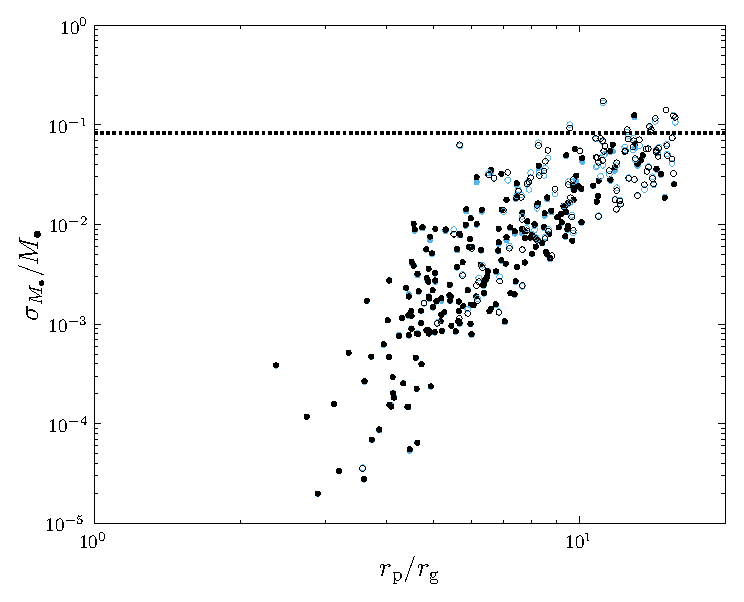
\includegraphics[width=0.475\textwidth]{./images/Fig_MW_MCMC_sigmas_rp_1}} \quad
\subfigure[MBH mass $M_\bullet$ versus SNR.]{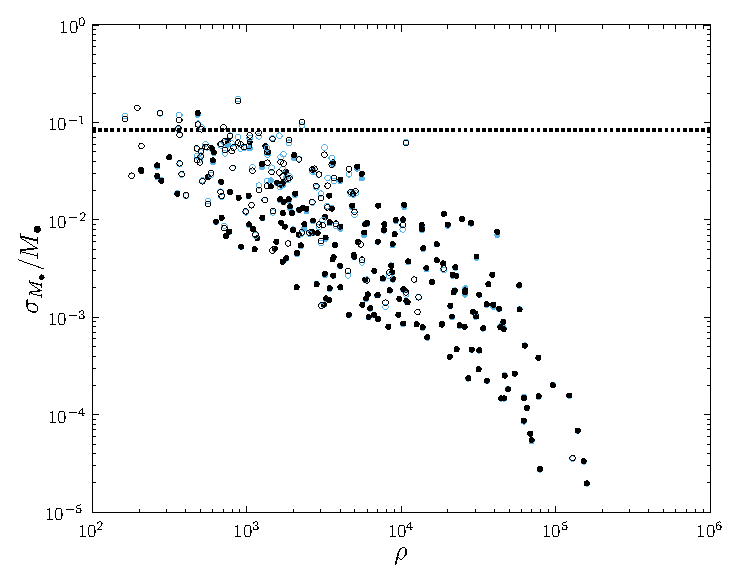
\includegraphics[width=0.485\textwidth]{./images/Fig_MW_MCMC_sigmas_SNR_1}} \\
\subfigure[MBH spin $a_\ast$ versus periapsis.]{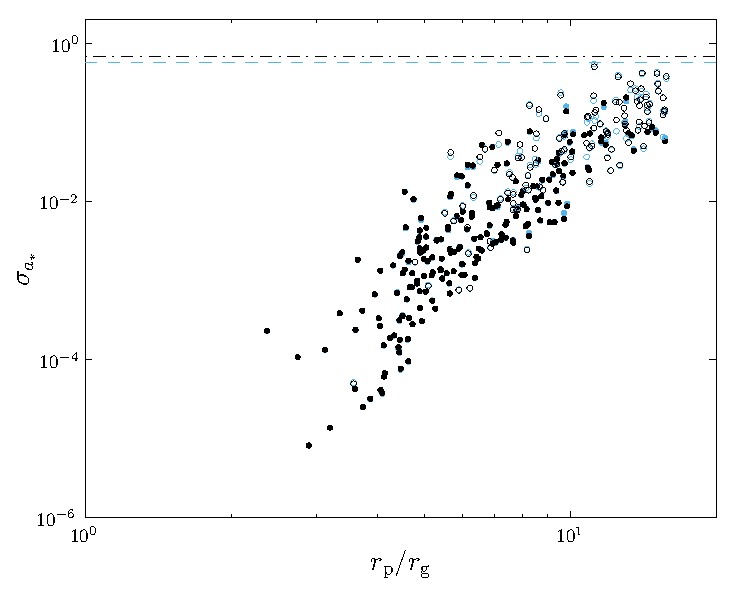
\includegraphics[width=0.475\textwidth]{./images/Fig_MW_MCMC_sigmas_rp_2}} \quad
\subfigure[MBH spin $a_\ast$ versus SNR.]{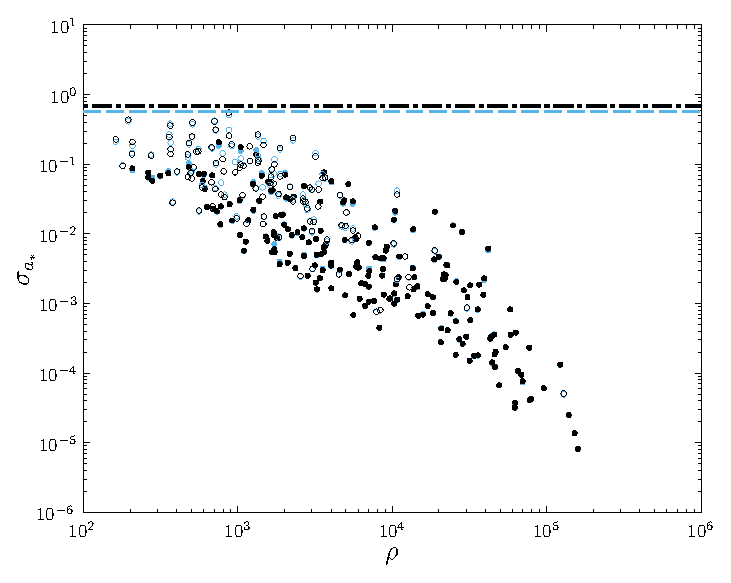
\includegraphics[width=0.485\textwidth]{./images/Fig_MW_MCMC_sigmas_SNR_2}} \\
\subfigure[Orientation angle $\Theta\sub{K}$ versus periapsis.]{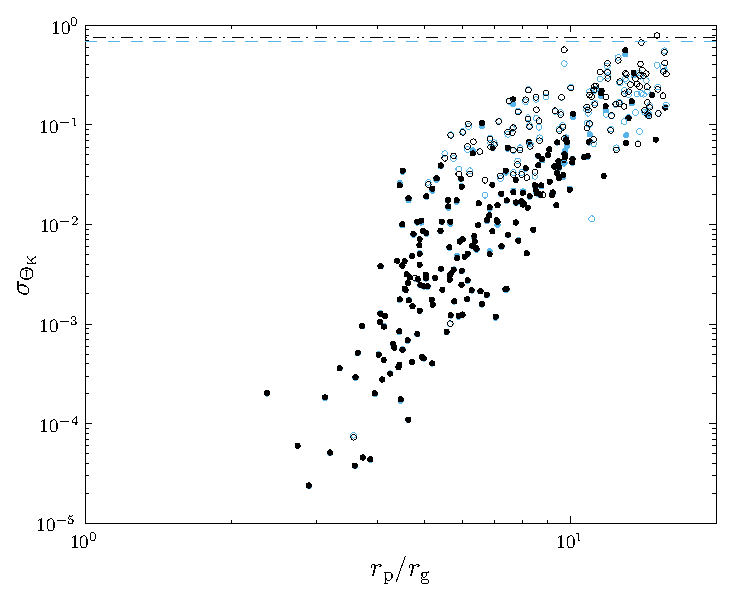
\includegraphics[width=0.475\textwidth]{./images/Fig_MW_MCMC_sigmas_rp_8}} \quad
\subfigure[Orientation angle $\Theta\sub{K}$ versus SNR.]{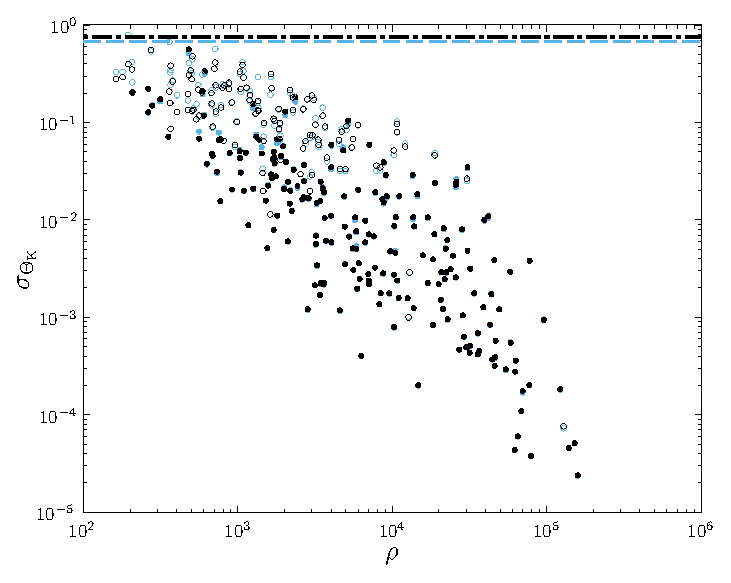
\includegraphics[width=0.485\textwidth]{./images/Fig_MW_MCMC_sigmas_SNR_8}}
\caption{Distribution widths as functions of periapsis $r\sub{p}$ and SNR $\rho$. The light blue points are used for the standard deviation, the black for the $68$-percentile half-width. The filled circles are converged runs and the open circles for those yet to converge. The dotted line is the current uncertainty for $M_\bullet$. The dashed line is the standard deviation for an uninformative prior and the dot--dashed line is the equivalent $68$-percentile half-width.\label{fig:sigmas}}
\end{center}
\end{figure}
\begin{figure}%[!htp]
\setcounter{subfigure}{6}
\begin{center}
\subfigure[Orientation angle $\Phi\sub{K}$ versus periapsis.]{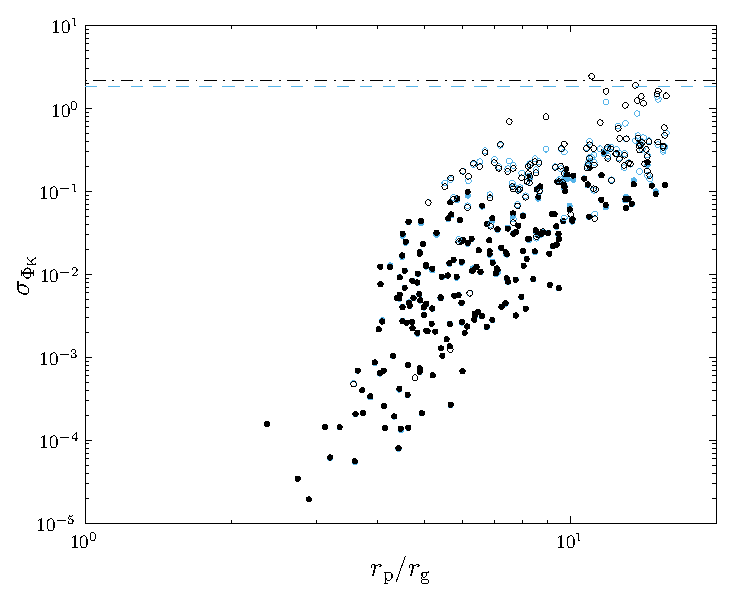
\includegraphics[width=0.475\textwidth]{./images/Fig_MW_MCMC_sigmas_rp_9}} \quad
\subfigure[Orientation angle $\Phi\sub{K}$ versus SNR.]{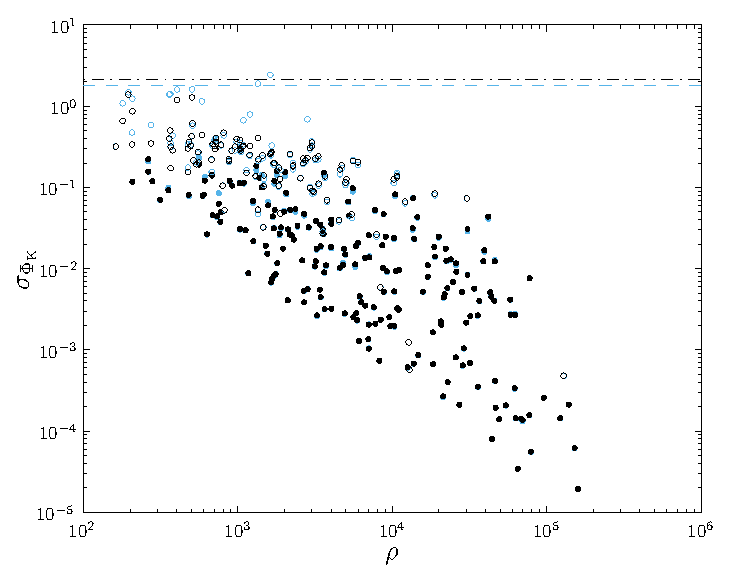
\includegraphics[width=0.485\textwidth]{./images/Fig_MW_MCMC_sigmas_SNR_9}} \\
\subfigure[Scaled distance $\zeta$ versus periapsis.]{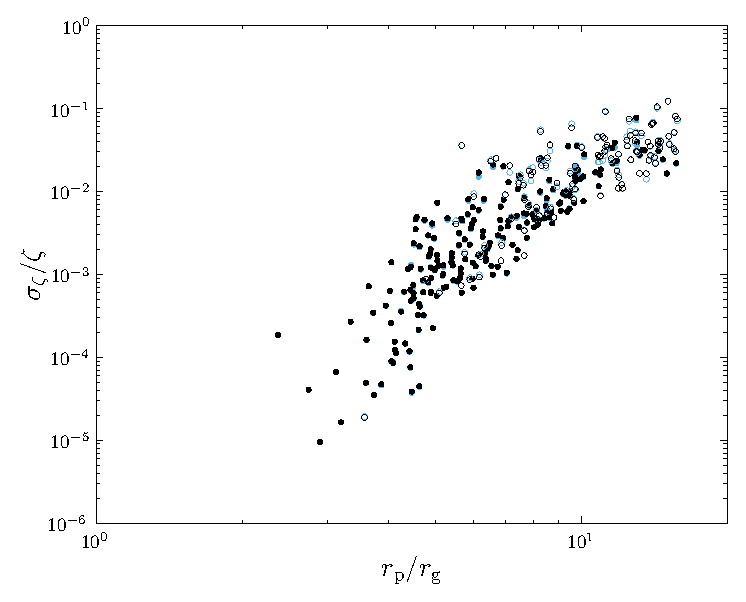
\includegraphics[width=0.475\textwidth]{./images/Fig_MW_MCMC_sigmas_rp_10}} \quad
\subfigure[Scaled distance $\zeta$ versus SNR.]{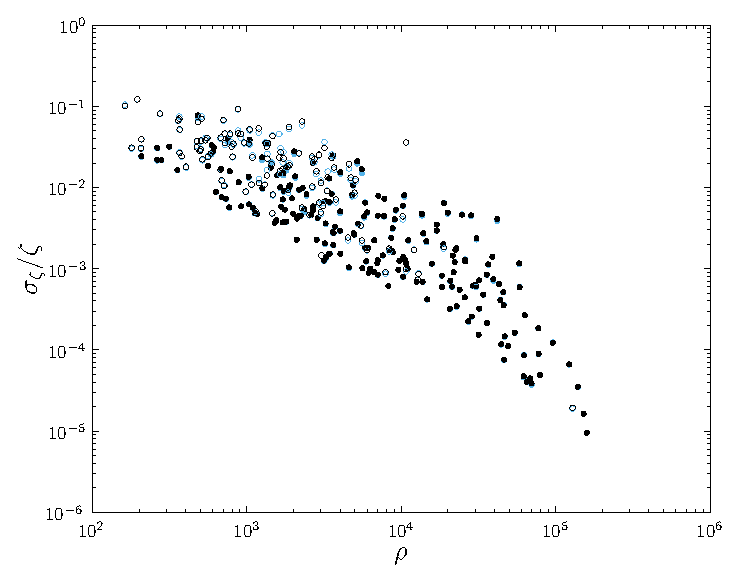
\includegraphics[width=0.485\textwidth]{./images/Fig_MW_MCMC_sigmas_SNR_10}} \\
\subfigure[Angular momentum $L_\infty$ versus periapsis.]{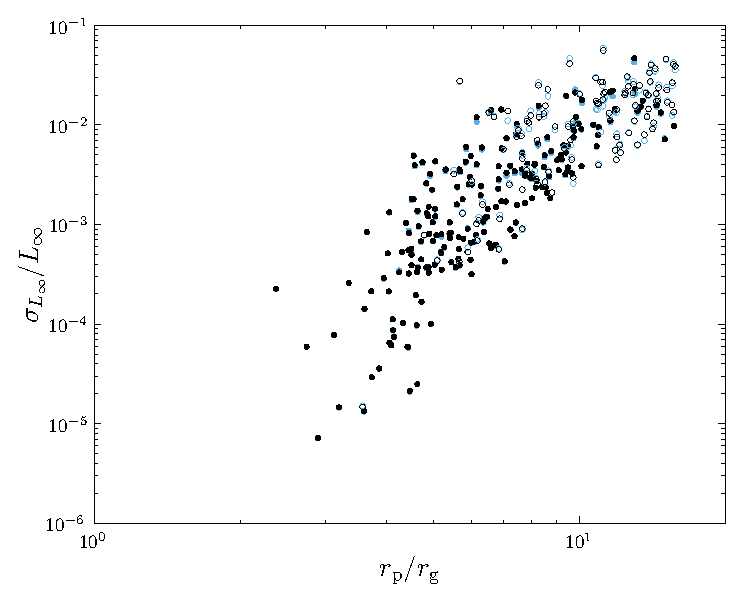
\includegraphics[width=0.475\textwidth]{./images/Fig_MW_MCMC_sigmas_rp_3}} \quad
\subfigure[Angular momentum $L_\infty$ versus SNR.]{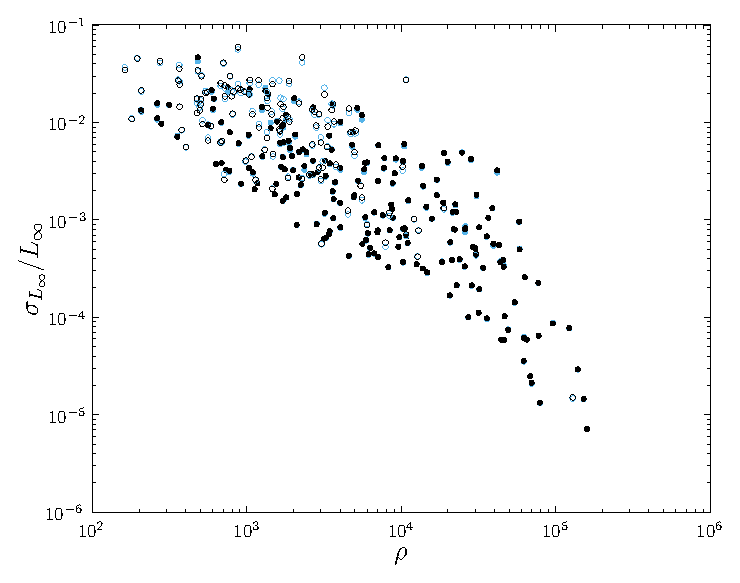
\includegraphics[width=0.485\textwidth]{./images/Fig_MW_MCMC_sigmas_SNR_3}} \\
\contcaption{{\bf{(Continued)}} Distribution widths as functions of periapse $r\sub{p}$ and SNR $\rho$.}
\end{center}
\end{figure}
\begin{figure}%[!htp]
\setcounter{subfigure}{12}
\begin{center}
\subfigure[Orbital inclination $\iota$ versus periapsis.]{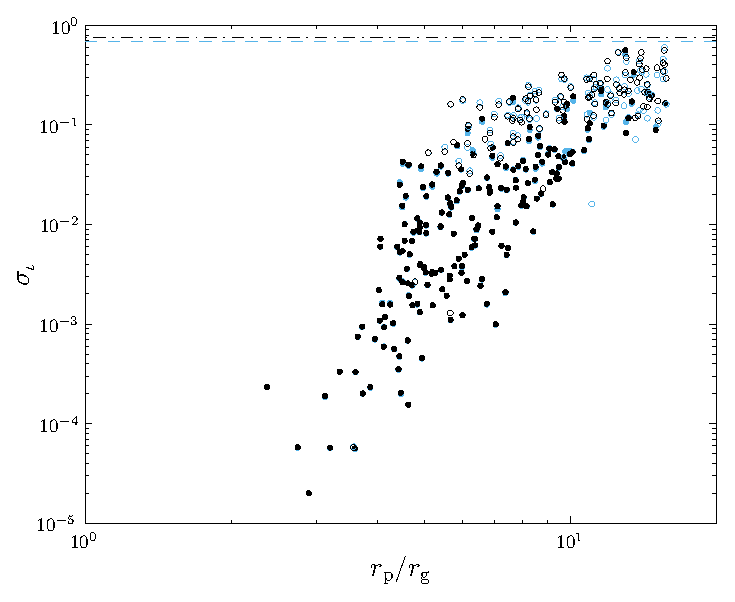
\includegraphics[width=0.475\textwidth]{./images/Fig_MW_MCMC_sigmas_rp_4}} \quad
\subfigure[Orbital inclination $\iota$ versus SNR.]{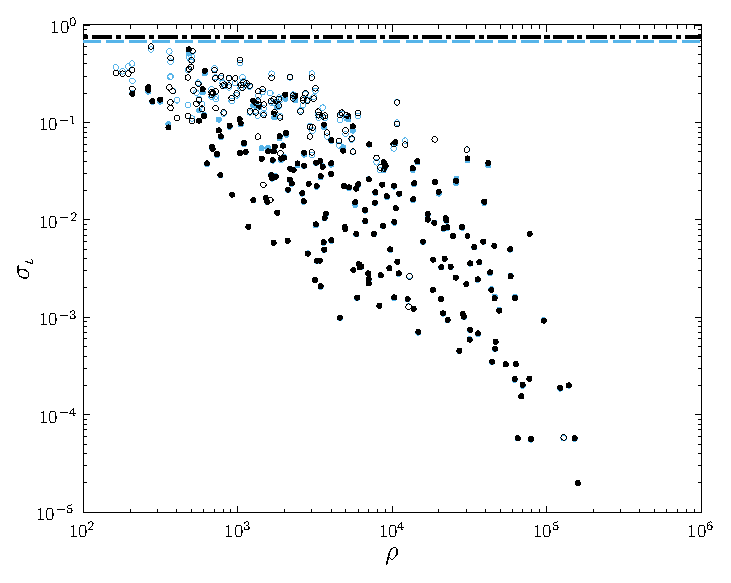
\includegraphics[width=0.485\textwidth]{./images/Fig_MW_MCMC_sigmas_SNR_4}} \\
\subfigure[Periapse azimuthal phase $\phi\sub{p}$ versus periapsis.]{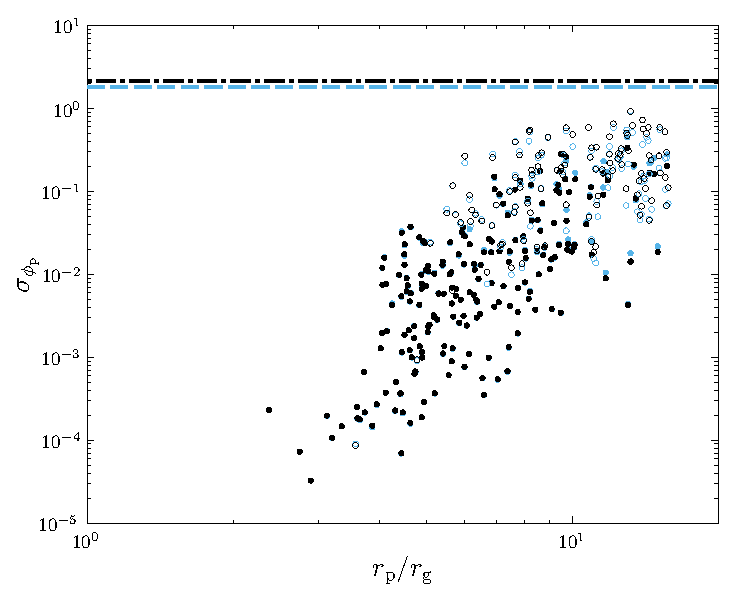
\includegraphics[width=0.475\textwidth]{./images/Fig_MW_MCMC_sigmas_rp_7}} \quad
\subfigure[Periapse azimuthal phase $\phi\sub{p}$ versus SNR.]{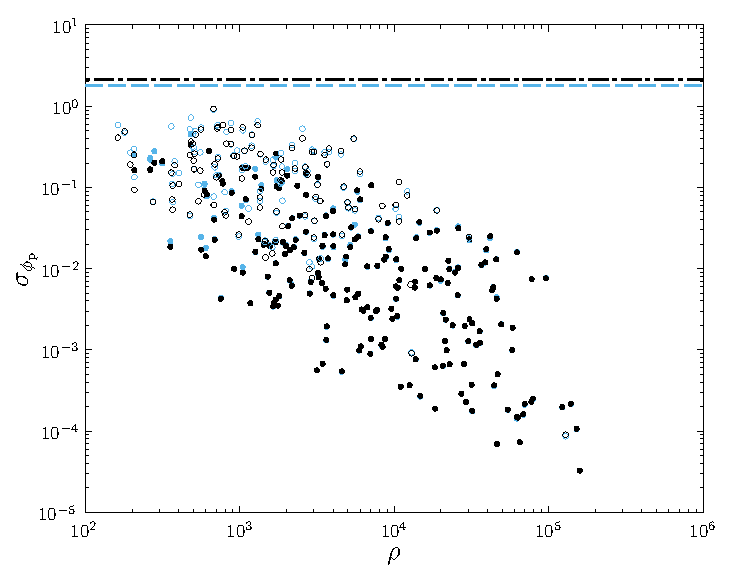
\includegraphics[width=0.485\textwidth]{./images/Fig_MW_MCMC_sigmas_SNR_7}} \\
\subfigure[Periapse polar phase $\chi\sub{p}$ versus periapsis.]{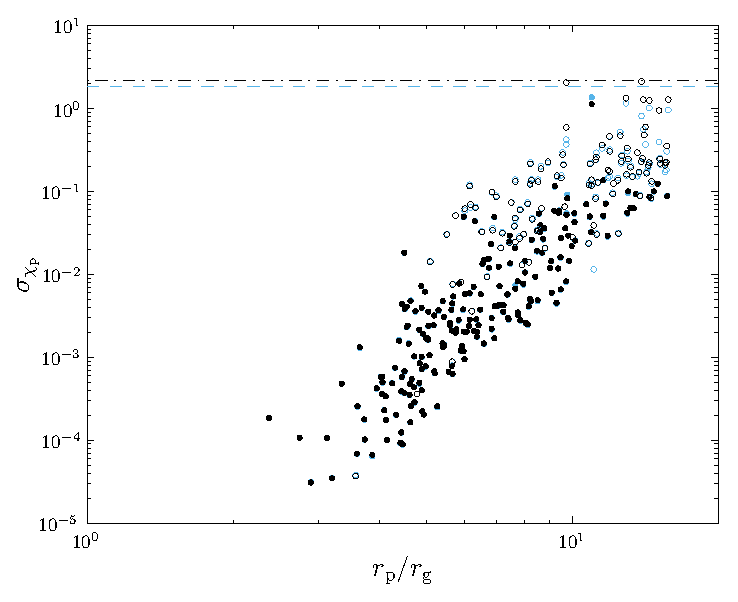
\includegraphics[width=0.475\textwidth]{./images/Fig_MW_MCMC_sigmas_rp_5}} \quad
\subfigure[Periapse polar phase $\chi\sub{p}$ versus SNR.]{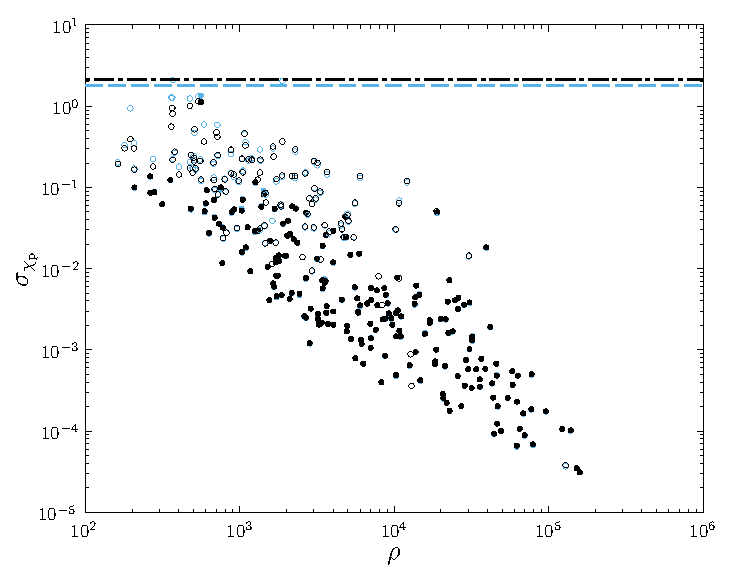
\includegraphics[width=0.485\textwidth]{./images/Fig_MW_MCMC_sigmas_SNR_5}} \\
\contcaption{{\bf{(Continued)}} Distribution widths as functions of periapse $r\sub{p}$ and SNR $\rho$.}
\end{center}
\end{figure}
\begin{figure}%[!htp]
\setcounter{subfigure}{18}
\begin{center}
\subfigure[Periapse time $t\sub{p}$ versus periapsis.]{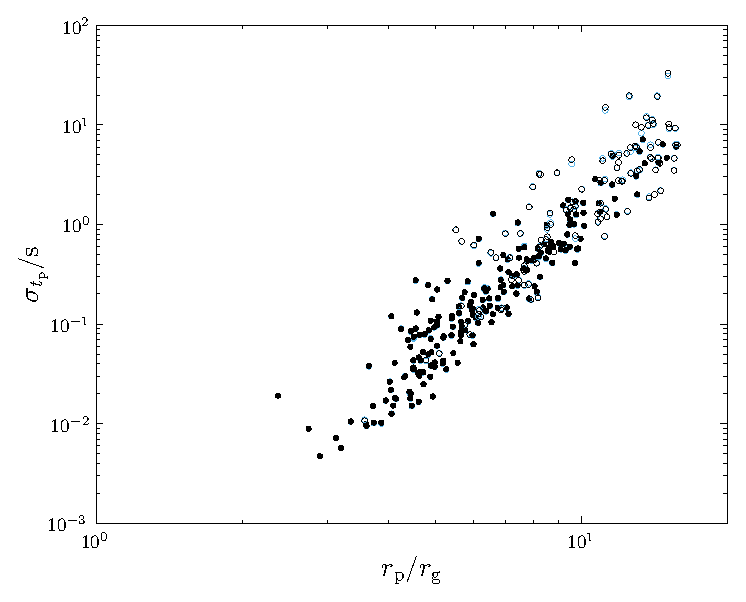
\includegraphics[width=0.475\textwidth]{./images/Fig_MW_MCMC_sigmas_rp_6}} \quad
\subfigure[Periapse time $t\sub{p}$ versus SNR.]{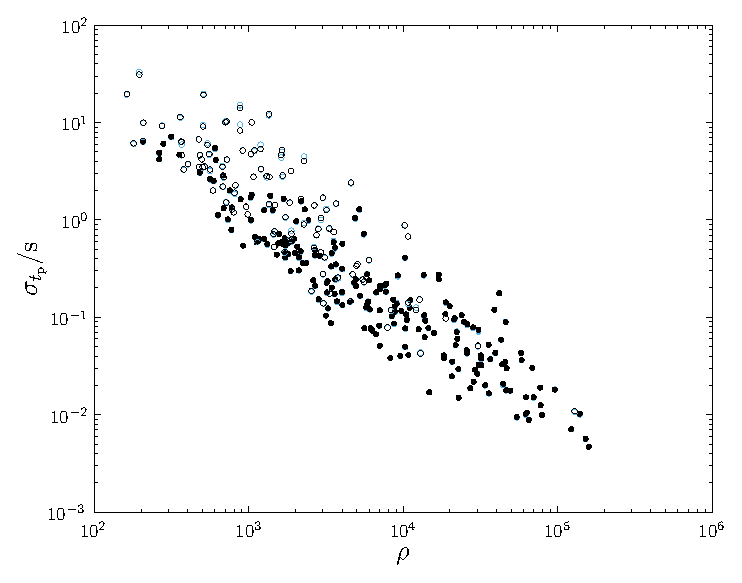
\includegraphics[width=0.485\textwidth]{./images/Fig_MW_MCMC_sigmas_SNR_6}} \\
\contcaption{{\bf{(Concluded)}} Distribution widths as functions of periapsis $r\sub{p}$ and SNR $\rho$.}
\end{center}
\setcounter{subfigure}{0}
\end{figure}
For guidance, the dotted line corresponds to the current measurement uncertainty for $M_\bullet$; the dashed lines are $\sigma\sub{SD}$ from uniform priors for $a_\ast$, $\Phi\sub{K}$, $\phi\sub{p}$, $\chi\sub{p}$, $\cos\Theta\sub{K}$ and $\cos\iota$, and the dot--dashed line are the equivalent $\sigma_{0.68}$. We have no expectations for the width of the MBH mass distribution with respect to the current value. However, we would expect that the recovered distributions for the other parameters are narrower than for the case of complete ignorance; this bound does seem to be respected. The two widths, $\sigma\sub{SD}$ and $\sigma_{0.68}$, typically agree better at smaller periapses and higher SNRs as would be expected for more Gaussian distributions.

The widths show a trend of decreasing with decreasing periapsis or increasing SNR, but there is a large degree of scatter. There does not appear to be a strong dependence upon any single input parameter, with the exception of the spin. The widths for $\iota$, $\Theta\sub{K}$, $\Phi\sub{K}$, $\phi\sub{p}$ and $\chi\sub{p}$ increase for smaller spin magnitudes. The dependence is shown in \figref{sigmas-spin}.
\begin{figure}%[!htp]
\begin{center}
\subfigure[MBH spin $a_\ast$.]{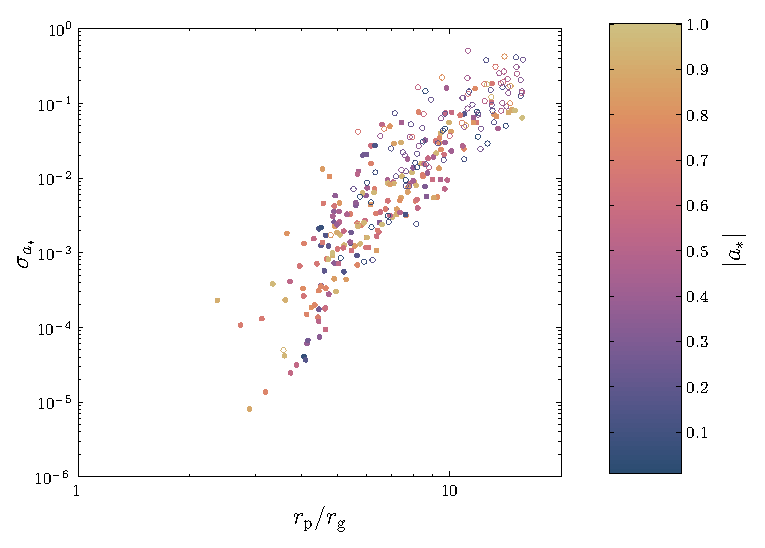
\includegraphics[width=0.48\textwidth]{./images/Fig_MCMC_sigmas_rp_spin_2}} \quad
\subfigure[Orientation angle $\Theta\sub{K}$.]{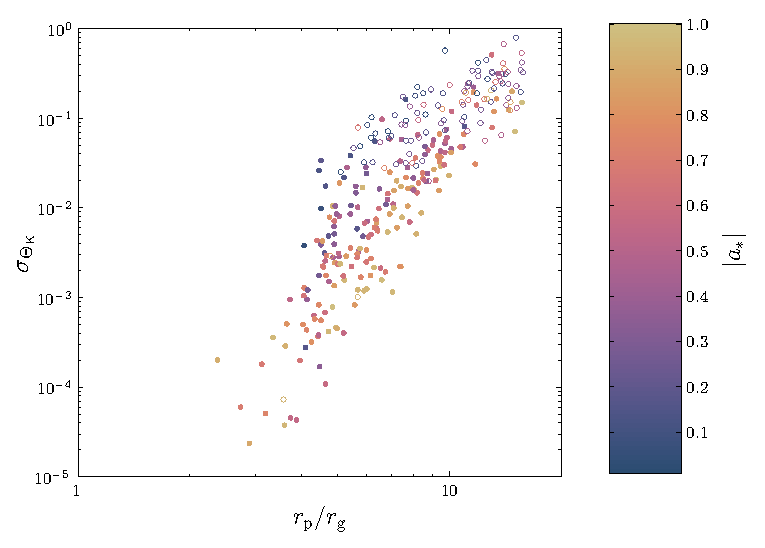
\includegraphics[width=0.48\textwidth]{./images/Fig_MCMC_sigmas_rp_spin_8}} \\
\subfigure[Orientation angle $\Phi\sub{K}$.]{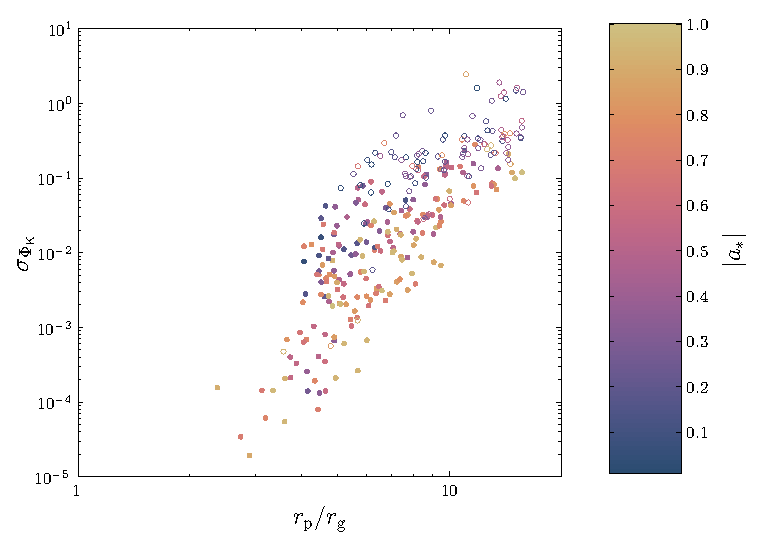
\includegraphics[width=0.48\textwidth]{./images/Fig_MCMC_sigmas_rp_spin_9}} \quad
\subfigure[Orbital inclination $\iota$.]{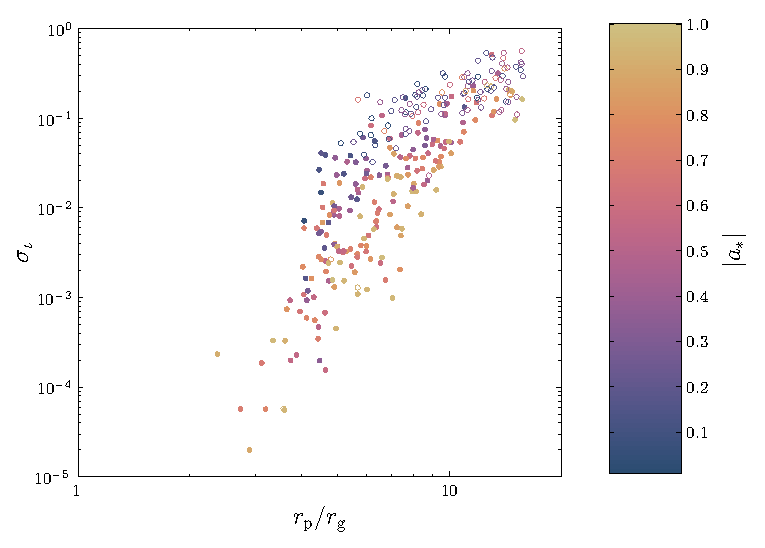
\includegraphics[width=0.48\textwidth]{./images/Fig_MCMC_sigmas_rp_spin_4}} \\
\subfigure[Periapse azimuthal phase $\phi\sub{p}$]{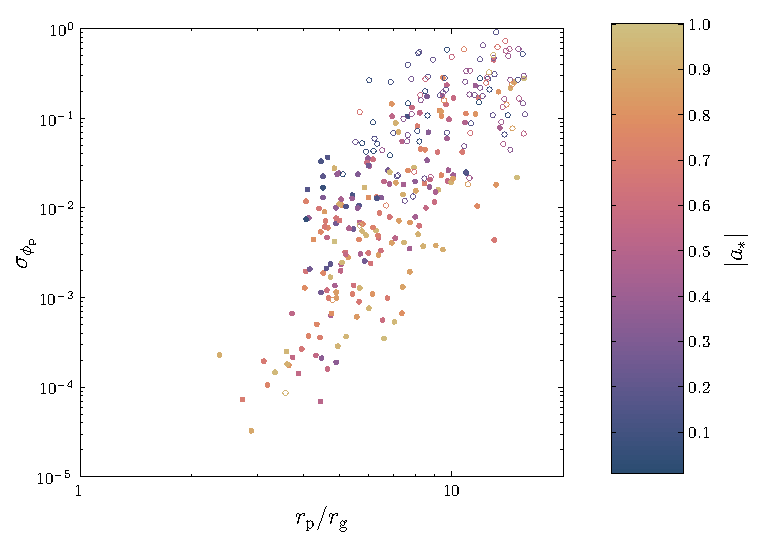
\includegraphics[width=0.48\textwidth]{./images/Fig_MCMC_sigmas_rp_spin_7}} \quad
\subfigure[Periapse polar phase $\chi\sub{p}$.]{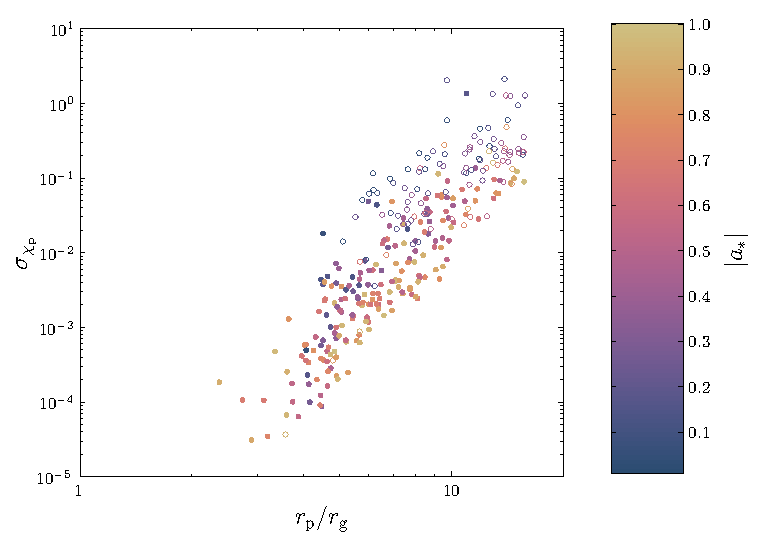
\includegraphics[width=0.48\textwidth]{./images/Fig_MCMC_sigmas_rp_spin_5}}
\caption{Parameter standard deviations versus periapsis $r\sub{p}$, showing dependence (or lack thereof) upon the spin magnitude $|a_\ast|$.\label{fig:sigmas-spin}}
\end{center}
\end{figure}
These parameters are defined with reference to the coordinate system established by the spin axis: for $a_\ast = 0$ we have spherical symmetry and there would be ambiguity in defining them. Therefore, it makes sense that they can be more accurately determined for larger spin magnitudes. The width for $a_\ast$, however, shows no clear correlation.

Comparing our MCMC and FIM results, we see there can be significant differences. Most parameters give results consistent to within an order (or two) of magnitude. The best agreement is for $t\sub{p}$, which is largely uncorrelated with the other parameters. The widths for $M_\bullet$, $a_\ast$, $L_\infty$ and $\iota$ show more severe differences; these parameters show the tightest degeneracies. The two methods do show signs of slowly converging with increasing SNR, as expected.

As a consistency check, to verify that the mismatch between the FIM and MCMC results is a consequence of parameter correlations, we calculated one-dimensional FIMs, only varying the MBH mass, and compared these to widths computed from MCMCs only sampling in mass. These were found to be in good agreement. The majority ($\sim 87\%$) have standard deviations consistent to within a factor of two; the rest within an order of magnitude.\footnote{One differed by more than an order of magnitude, and also failed to fulfil the (one dimensional) MM criterion; this was a numerical problem in calculating the FIM.} Some small difference is expected because of numerical error from calculating derivatives for the FIM by finite differencing.

\subsection{Scientific potential}

Having quantified the precision with which we could infer parameters from an EMRB waveform, we can now consider if it is possible to learn anything new.

Of paramount interest are the MBH mass and spin. The current uncertainty in the mass is $\sigma_{M_\bullet} = 0.36 \times 10^6 M_\odot$ ($\sim 8\%$; \citealt{Gillessen2009}). There are few runs amongst our data set that are not better than this: it appears that orbits of a $\mu = 10 M_\odot$ CO with periapses $r\sub{p} \lesssim 13 r\sub{g}$ should be able to match our current observational constraints. However, the EMRB is an independent measurement, and so a measurement of comparable precision to the current bound can still be informative. Accuracy of $1\%$ could be possible if $r\sub{p} \lesssim 8 r\sub{g}$.

The spin is less well constrained. To obtain an uncertainty for the magnitude of $0.1$, comparable to that achieved in X-ray measurements of active galactic nuclei, it appears that the periapsis needs to be $r\sub{p} \lesssim 11 r\sub{g}$. For smaller periapses, the uncertainty can be much less, indicating that an EMRB could be an excellent probe. The orientation angles for the spin axis may be constrained to better than $0.1$ for $r\sub{p} \lesssim 11 r\sub{g}$. It may well be possible to learn both the direction and the magnitude of the spin. This could illuminate the MBH's formation.

We have no {\it a priori} knowledge about the CO or its orbit, so anything we learn would be new. However, this is not particularly useful information, unless we observe multiple bursts, and can start to build up statistics for the dynamics of the GC. Using current observations for the distance to the GC, which could be further improved by the mass measurement from the EMRB, it is possible to infer a value for the mass $\mu$ from $\zeta$. This could inform us of the nature of the object (BH, NS or WD) and be a useful consistency check. A small value of $\zeta$, indicating a massive CO, is unambiguous evidence for the existence of a stellar-mass BH.

\section{Summary and conclusions}

We have analysed the properties of EMRBs from the Galactic Centre. We used NK waveforms built used spherical polar and oblate spheroidal coordinates. The two coordinate schemes yield almost indistinguishable results. There may be differences when the spin is large and the periapse is small: $\sim 10\%$ for $r\sub{p} \simeq 4 r\sub{g}$, $\sim 20\%$ for $r\sub{p} \simeq 2 r\sub{g}$. This is less than the error inheritant in the semirelativistic approximation infered from the difference in NK and BH perturbation theory energy fluxes in \secref{Energy}. We conclude that either is a valid choice for this purpose and have adopted spherical polar coordinates.

The SNR of bursts is well correlated with the periapsis, it can be reasonably described as having a power-law dependence. Using LISA, signals should be detectable for a $1 M_\odot$ ($10 M_\odot$) object if the periapse is $r\sub{p} < 27 r\sub{g}$ ($r\sub{p} < 65 r\sub{g}$), corresponding to a physical scale of $1.7 \times 10^{11}\units{m}$ ($4.1 \times 10^{11}\units{m}$) or $5.6 \times 10^{-6}\units{pc}$ ($1.3 \times 10^{-5}\units{pc}$). Using eLISA, these distances are approximately approximately three times smaller.

We conducted an investigation using Fisher matrix analysis into how precisely we could infer parameters of the GC's MBH. However, we found that the linearised-signal approximation does not hold for these bursts over a wide range of SNR. This demonstrates the necessity of checking the approximation before quoting the results of an analysis \citep{Vallisneri2008}.

We used MCMC results as a more robust measure of parameter estimation accuracy. Potentially, it is possible to determine very precisely the key parameters defining the MBH's mass and spin, if the orbit gets close enough to the MBH. It appears that we can achieve good results from a single EMRB with periapsis of $r\sub{p} \simeq 10 r\sub{g}$ for a $10 M_\odot$ CO. This translates to a distance of $6 \times 10^{10}\units{m}$ or $2 \times 10^{-6}\units{pc}$. Orbits closer than this would place stricter constraints. The best orbits yield uncertainties of almost one part in $10^5$ for the MBH mass and spin, far exceeding existing techniques. Conversely, orbits with $r\sub{p} \gtrsim 16 r\sub{g}$ are unlikely to provide any useful information.

Before we can quote results for how accurately we can determine the various parameters, we must consider the probability of each orbit. This shall be done in ....

We have so far only considered EMRBS from our Galaxy, a natural extension is to consider bursts from extragalactic sources, which do in the next chapter. Extragalactic bursts are not as promising as those from the GC, but could still make a significant contribute to the total burst event rate. 